89. Для построения графика функции $f(x)=|x^2+2x-3|$ сначала построим параболу $y=x^2+2x-3=(x-1)(x+3).$ После этого отразим её отрицательную часть при $x\in(-3;1)$ наверх относительно оси абсцисс. Её вершина $(-1;-4)$ отразится в точку $(1;4).$ График функции $g(x)=k(x+5)+4$ при любом значении $k$ проходит через точку $(-5;4).$  С графиком функции $f(x)$ он может иметь три общие точки только в двух случаях: если параллелен оси абсцисс, тогда $k=0,$ или если проходит через точку $(1;0),$ в этом случае $0=k\cdot6+4,\ k=-\cfrac{2}{3}.$
$$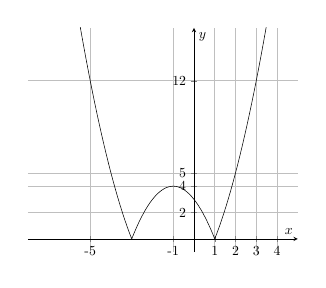
\begin{tikzpicture}[scale=0.5]
\begin{axis}[
    axis lines = middle,
    grid=major,
    legend pos={south west},
    xlabel = {$x$},
    %xlabel style={below right},
    ylabel = {$y$},
    ymin=-1,
    ymax=16,
    xmin=-8,
    xmax=5,
    xtick={-5,-1,1,2,3,4},
    xticklabels={-5,-1,1,2,3,4},
    ytick={2,4,5,12},
    yticklabels={2,4,5,12},
                  ]
	\addplot[domain=-6:5, samples=100, color=black] {abs(x*x+2*x-3)};
        %\addplot[domain=2.01:6, samples=100, color=black] {2/(2-x)};
   % \addplot[domain=-3:3, samples=100, color=black] {-x};
     %\addlegendentry{$\text{Рис. 1}$};
\end{axis}
\end{tikzpicture}$$
